\chapter{Progettazione e sviluppo}\label{chapter:progettazionesviluppo}
In questo capitolo saranno esposti gli approcci teorici e pratici per lo sviluppo del progetto.


\section{Introduzione ai microservizi}\label{sec:microserviziintro}
Prima di introdurre il concetto di architettura a microservizi è bene introdurre il concetto di architettura monolitica.\\
Un’architettura monolitica è una metodologia di sviluppo secondo la quale tutti i processi coinvolti sono strettamente legati tra di loro e sono erogati come un singolo servizio.\\
Questa tipologia di approccio porta ad avere sistemi nei quali modificare le funzionalità diventa più complesso in quanto si deve agire sull’intero sistema e non solo sulle parti effettivamente interessate.\\
Inoltre, utilizzare un’architettura monolitica porta a correre dei rischi per quanto riguarda la disponibilità dell’applicazione, in quanto anche se solo uno dei processi coinvolti avesse un malfunzionamento, questo si propagherebbe nell’intera applicazione.\\ \\
Per quanto riguarda le architetture a microservizi, queste sono diametralmente opposte alle architetture monolitiche.\\
Nelle architetture a microservizi l’obiettivo è quello di scomporre l’applicazione da realizzare nelle sue funzioni (\emph{servizi}) di base.\\
Ogni servizio può essere compilato e distribuito in modo indipendente; quindi i singoli servizi possono funzionare o non funzionare senza compromettere gli altri.\\
Utilizzare i microservizi significa riuscire a gestire criticità inevitabili, poter sfruttare la scalabilità dinamica e semplificare l'integrazione di nuove caratteristiche.\\

\begin{figure}[ht]
	\centering
	\resizebox{1.0\textwidth}{!}{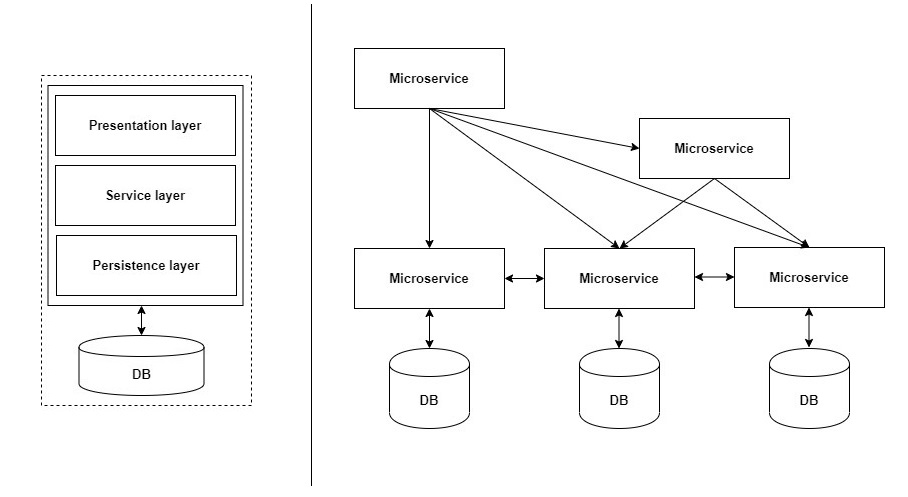
\includegraphics{img/monovsmicro}}
	\caption{Architettura monolitica e architettura a microservizi a confronto}
	\label{fig:one}
\end{figure}

Oggi i container Linux permettono di eseguire più parti di un'applicazione in modo indipendente con un controllo superiore sui singoli componenti.\\
I microservizi containerizzati rappresentano la base delle applicazioni cloud native.\\ \\
Di seguito sono elencati alcuni dei vantaggi di un’architettura a microservizi:

\begin{itemize}
	\item \textbf{Agilità}\\ Essendo ogni applicazione suddivisa in servizi di base, i team di sviluppo agiscono in contesti ridotti, semplificando il lavoro e ridurre i tempi del ciclo di sviluppo.
	\item \textbf{Scalabilità}\\Lavorare con un microservizio consente di scalare in modo indipendente per rispondere alla richiesta di un determinato servizio.\\ In questo modo è possibile misurare il carico di lavoro di un singolo servizio e adattarlo di conseguenza; il che può portare a dei vantaggi anche in termini economici per il mantenimento dell’applicazione. 
	\item \textbf{Semplicità di distribuzione}\\ I microservizi supportano l’approccio \emph{CI/CD} (Continuous integration/Continuous Delivery), così da semplificare l’integrazione e il testing di nuove funzionalità avendo comunque la possibilità di effettuare un rollback in caso di problemi.
	\item \textbf{Codice riutilizzabile}\\ Uno dei vantaggi del suddividere un’applicazione in servizi è la possibilità di poter riutilizzare codici di servizi già esistenti per altre applicazioni.
	\item \textbf{Resilienza}\\ Avendo un’applicazione a servizi indipendenti si aumenta la resilienza in caso di errori.\\ Si possono gestire completamente gli errori di un servizio isolando la funzionalità senza bloccare l’intera applicazione.
\end{itemize}

\section{Il microservizio \texttt{CheckEmail}}\label{sec:architetturamicroservizio}
Il microservizio realizzato verifica l'avvenuto acquisto di un modulo applicativo da parte di un utente, identificato, ai fini del microservizio, da un indirizzo e-mail.\\
Lo scopo principale del microservizio è quello di ricevere una richiesta \texttt{HTTP} con all’interno del body un indirizzo e-mail.\\
Una volta estratto l’indirizzo e-mail il microservizio effettua una \emph{query} all’interno del Database per controllare che l’indirizzo sia presente nella tabella degli utenti abilitati all’utilizzo di un determinato servizio.\\
In base al risultato della query il microservizio restituisce un codice \texttt{HTTP} come risposta alla richiesta.\\
\newline
La tipologia di richieste descritte sono effettuate tramite il metodo \textbf{\texttt{GET}} di \texttt{HTTP}, quindi vengono richiesti dei dati dal server.\\
\newpage
I codici che possono essere restituiti sono:\\
\begin{table}[ht]
	\centering
	\resizebox{1.0\linewidth}{!}{
		\begin{tabular}{|c|c|c|}
			\hhline{|-|-|-|}
			\textbf{Codice \texttt{HTTP}} & \textbf{Significato} & \textbf{Descrizione}\\
			\hhline{|-|-|-|}
			200 & OK & Il microservizio ha risposto correttamente \cr && e l'utente è autorizzato a procedere. \\
			\hhline{|-|-|-|}
			402 & PAYMENT REQUIRED & Il microservizio ha risposto correttamente \cr && ma l'utente non è autorizzato a procedere.\\
			\hhline{|-|-|-|}
			500 & INTERNAL SERVER ERROR & Messaggio di errore generico, \cr && non si è potuto raggiungere il microservizio.\\
			\hhline{|-|-|-|}
			503 & SERVICE UNAVAILABLE & Server non disponibile, \cr && non si è potuto raggiungere il microservizio. \\
			\hhline{|-|-|-|}
		\end{tabular}
	}
	\vspace*{2mm}
	\caption{Codici \texttt{HTTP} restituiti dal microservizio}
	\label{tab:httpcode}
\end{table}

\begin{figure}[ht]
	\centering
	\resizebox{0.9\textwidth}{!}{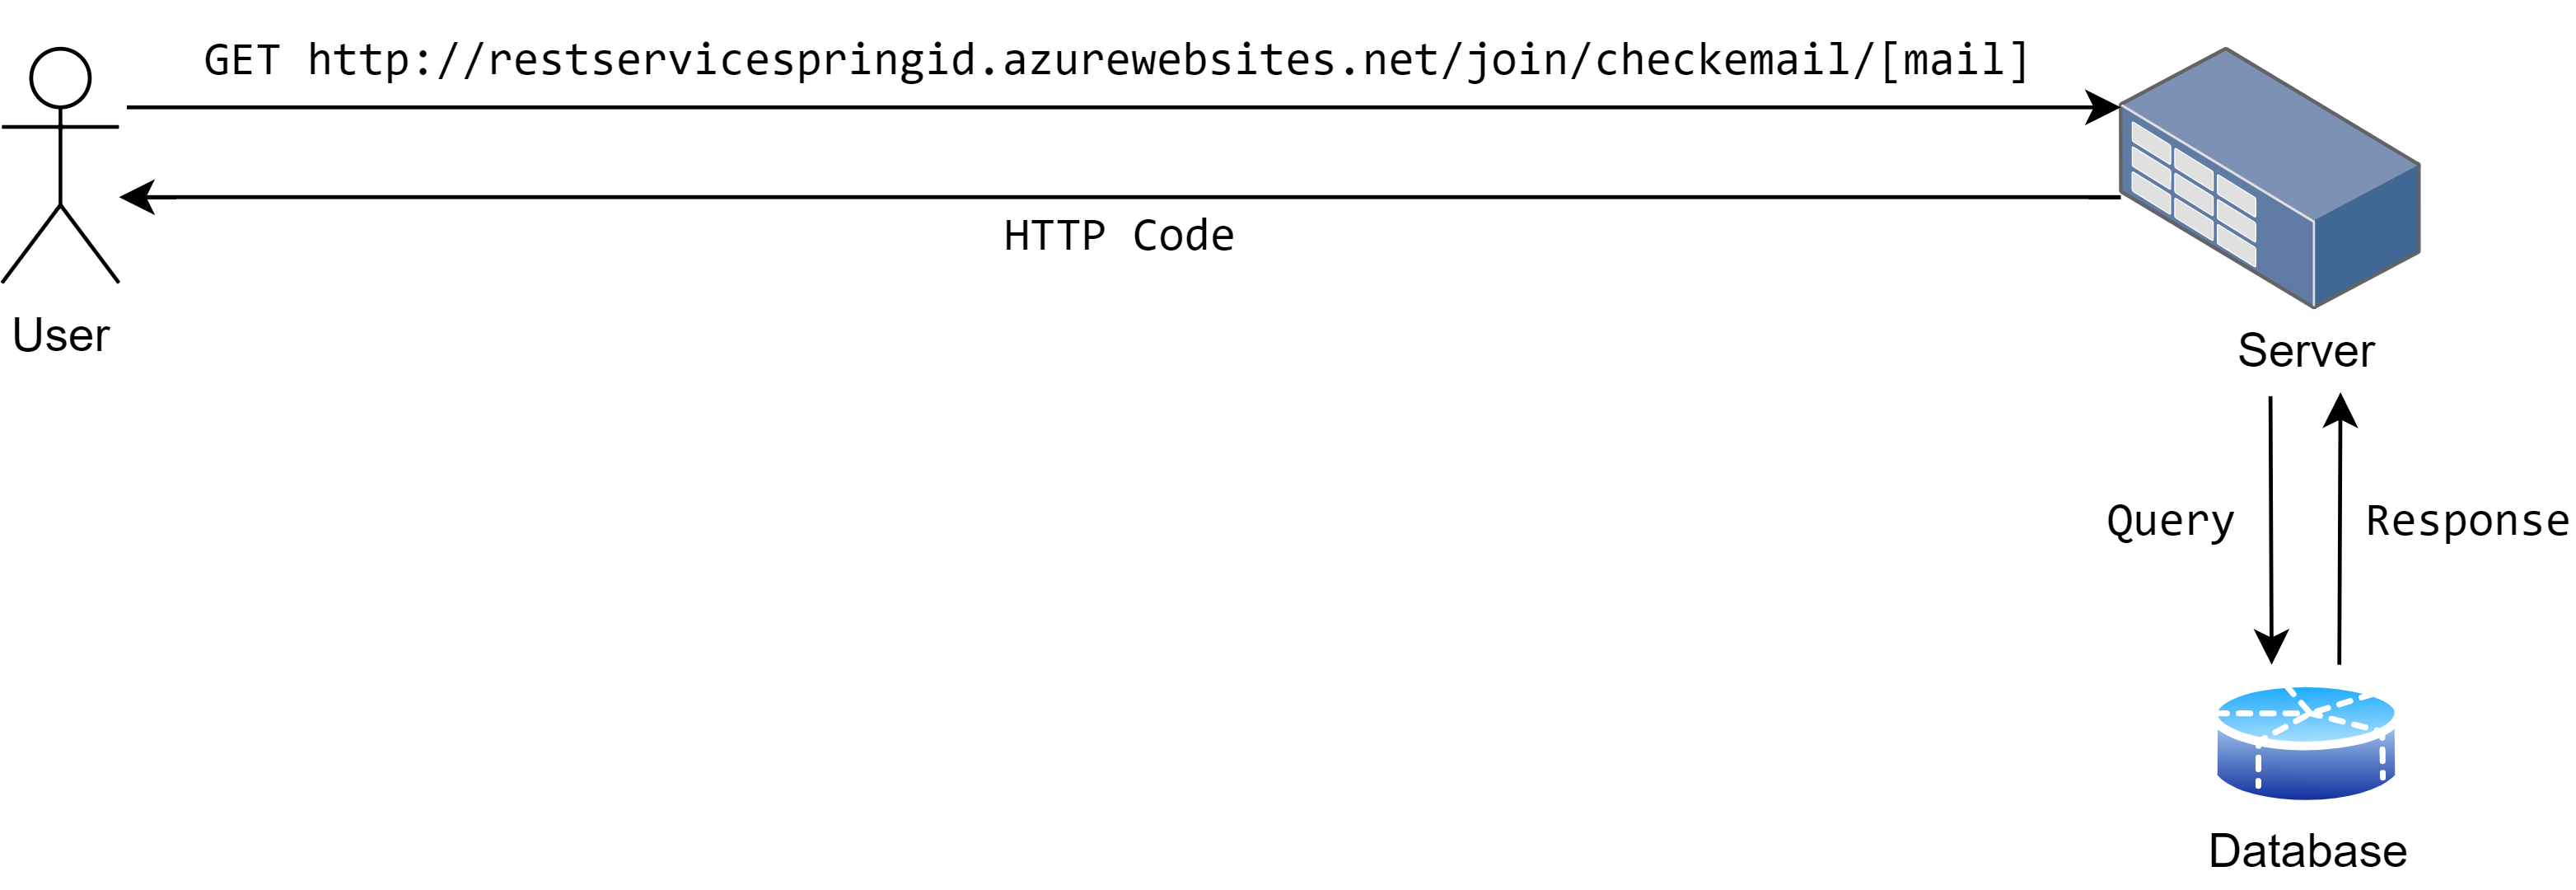
\includegraphics{img/comunicazionemicroservizio}}
	\caption{Schema di comunicazione Utente - microservizio}
	\label{fig:one}
\end{figure}

\subsection{Sviluppo}\label{sec:sviluppomicroservizio}
\subsubsection{Database}
Per sviluppare ed utilizzare il microservizio si è resa necessaria la creazione del Database PostgresSQL per la memorizzazione dei dati degli utenti.\\
È bene premettere che il Database è stato volutamente creato nella maniera più semplice e facilmente mantenibile possibile dato che durante lo sviluppo questo doveva servire solo per scopi di testing.\\
Il Database è composto da due tabelle:
\begin{itemize}
		\item \textbf{\texttt{users}}\\ Contiene le informazioni di tutti gli utenti abilitati ad accedere ad un determinato servizio.
		\item \textbf{\texttt{email}}\\ Contiene gli indirizzi e-mail di tutti gli utenti della piattaforma, quindi non è garantito che tutti avranno accesso a tutti i servizi.
\end{itemize}
\begin{figure}[ht]
	\centering
	\resizebox{0.3\textwidth}{!}{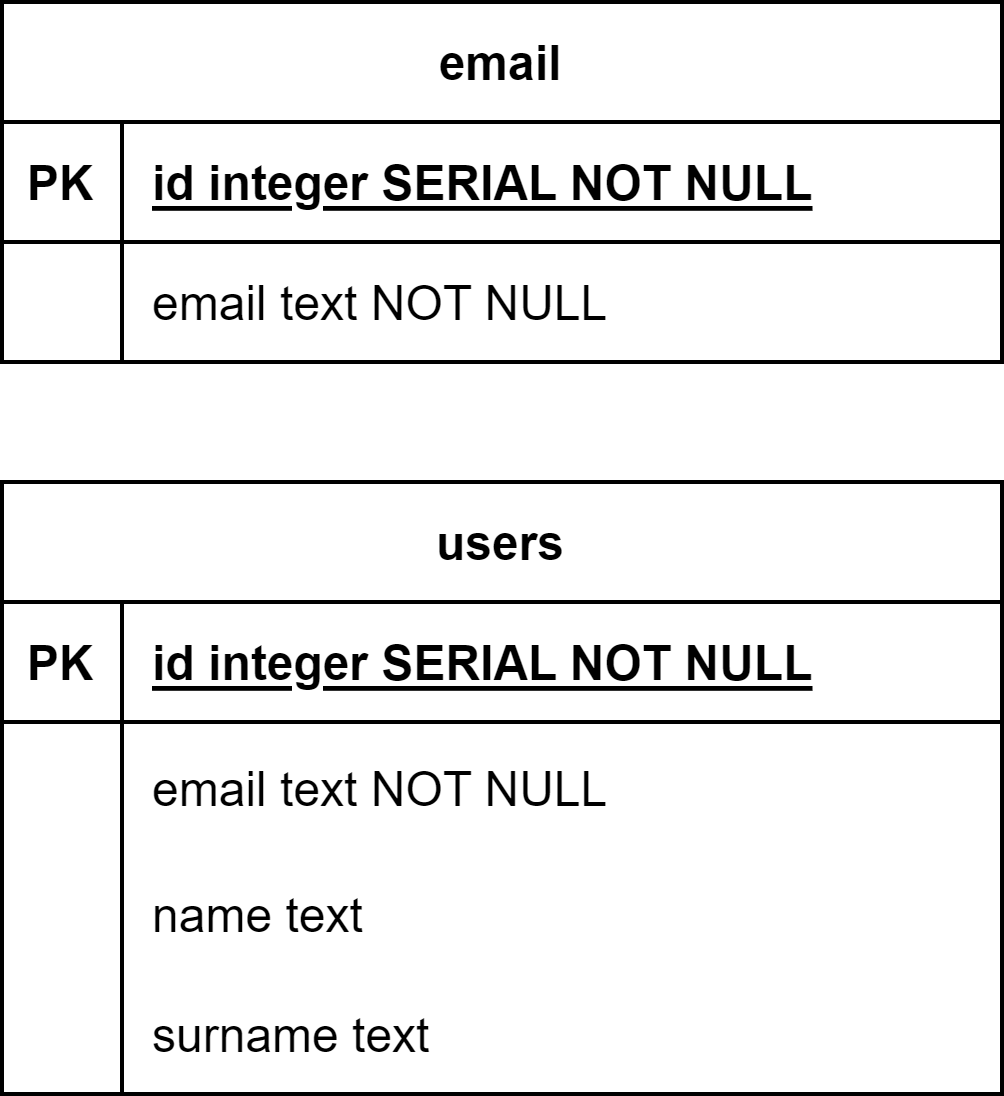
\includegraphics{img/dbtables-drawio}}
	\caption{Modello Entità Relazione del Database}
	\label{fig:one}
\end{figure}
% \begin{figure}[ht]
% 	\centering
% 	\resizebox{0.8\textwidth}{!}{\includegraphics{img/emaildb_e}}
% 	\caption{Contenuto delle tabelle visualizzato dalla shell di PostgresSQL}
% 	\label{fig:one}
% \end{figure}

\subsubsection{Microservizio}
Per lo sviluppo del microservizio, come accennato in precedenza, è stato deciso di utilizzare il linguaggio di programmazione Java e il framework Spring.\\
Il progetto è stato realizzato utilizzando l’IDE Eclipse ed è composto da cinque \emph{package}.
\begin{figure}[h]
	\centering
	\resizebox{0.6\textwidth}{!}{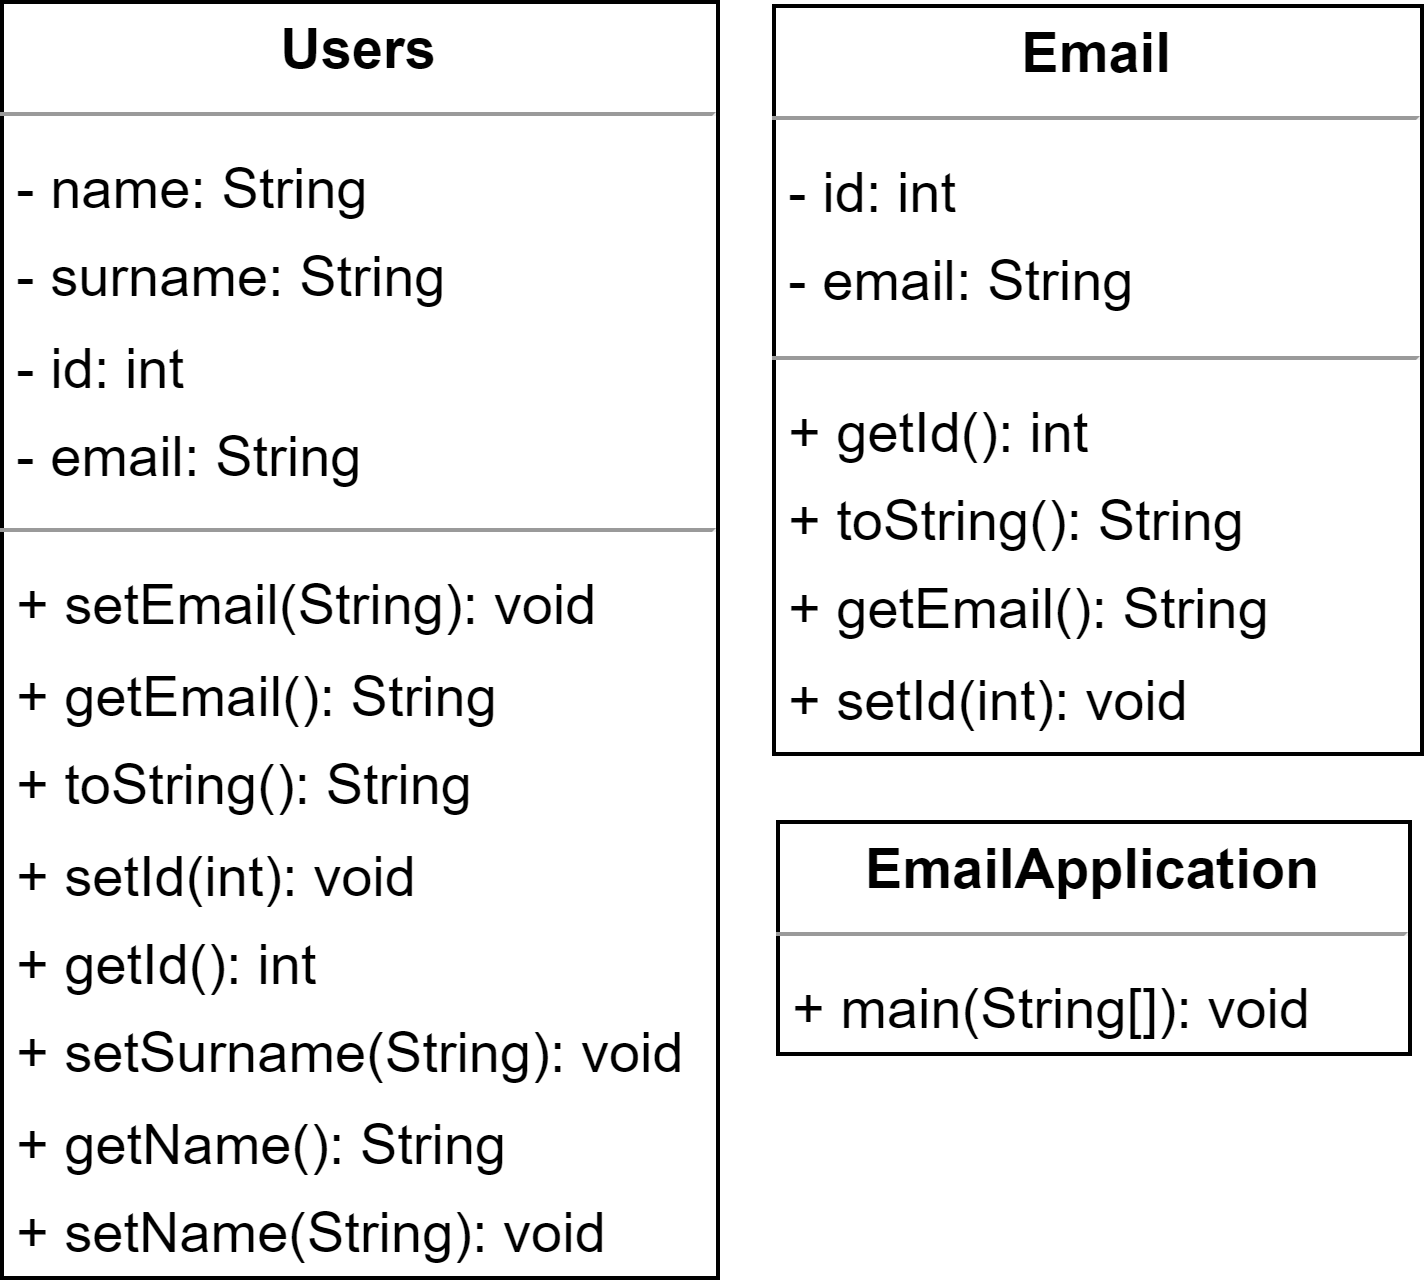
\includegraphics{img/classi}}
	\caption{Diagramma UML delle classi principali del progetto}
	\label{fig:one}
\end{figure}

\begin{figure}[h]
	\centering
	\resizebox{0.8\textwidth}{!}{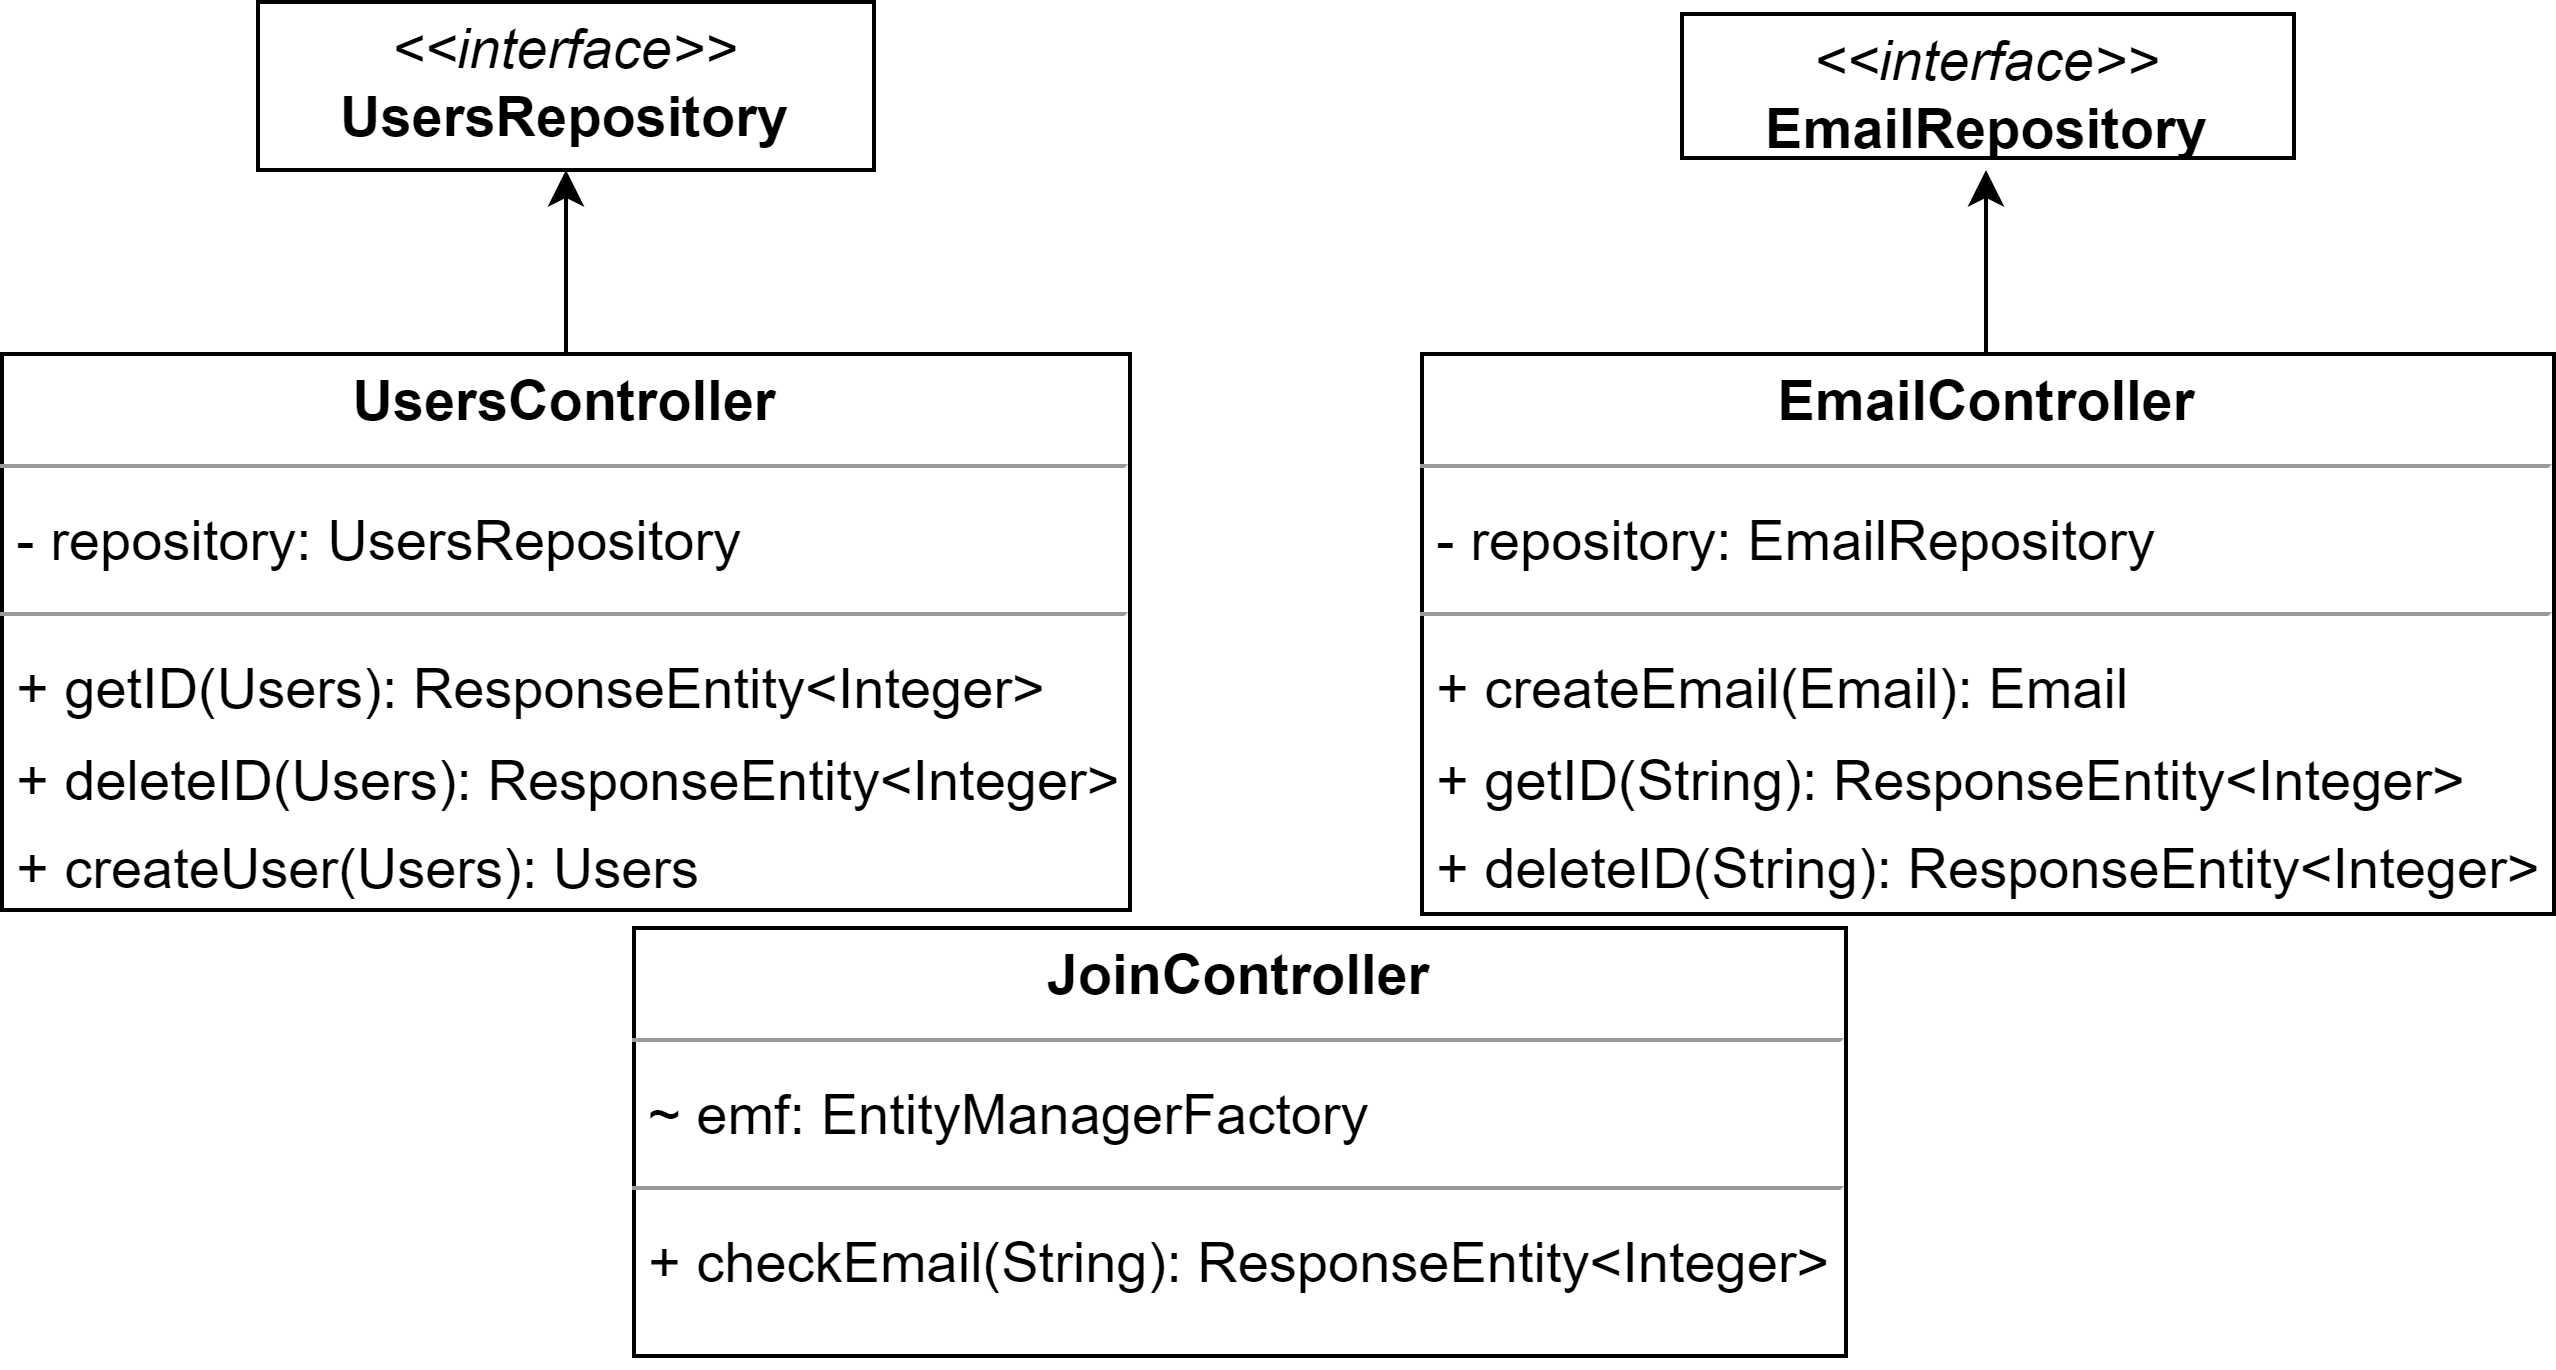
\includegraphics{img/controller}}
	\caption{Diagramma UML delle classi \emph{controller} del progetto}
	\label{fig:one}
\end{figure}
\newpage
\begin{figure}[h]
	\centering
	\resizebox{0.5\textwidth}{!}{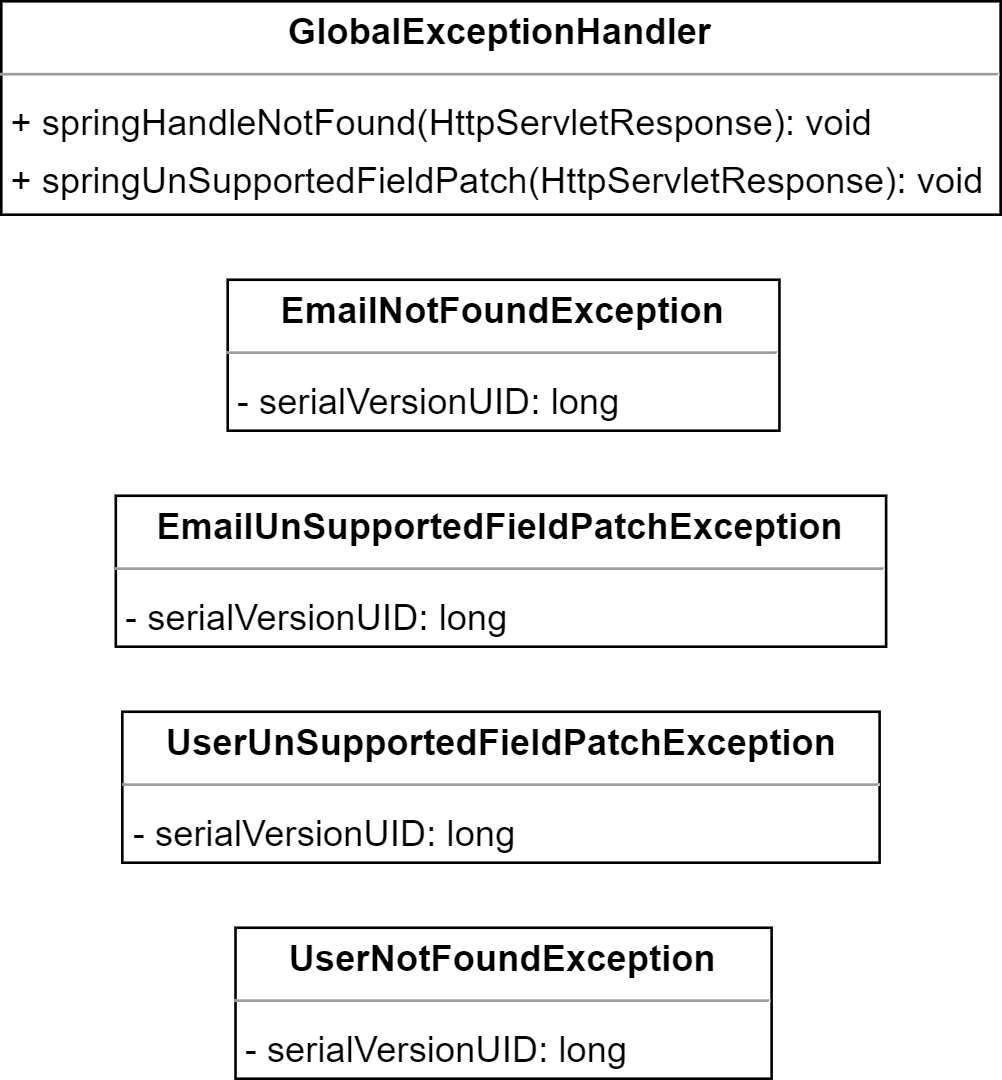
\includegraphics{img/exception}}
	\caption{Diagramma UML delle \emph{custom exception} del progetto}
	\label{fig:one}
\end{figure}

Descrizione dei package:
\begin{itemize}
	\item \textbf{\texttt{com.aesys.valeriodesiati.mail}}\\ Contiene la classe principale del microservizio.
	\item \textbf{\texttt{com.aesys.valeriodesiati.mail.model}}\\ Contiene le classi relative alle Entità all’interno del Database.\\ \emph{Spring Boot JPA} consente la creazione di entità in un Database a partire da una normale classe Java tramite l’aggiunta di annotazioni fornite dal framework.\\Un esempio di utilizzo di un \emph{model} è l'Algoritmo \ref{alg:checkemailmodel}.
	\item \textbf{\texttt{com.aesys.valeriodesiati.mail.repository}}\\ Contiene le interfacce relative alle entità del Database che ereditano l’interfaccia \mintinline{java}{JpaRepository<T,ID>}.\\ Tale interfaccia contiene le API per tutte le operazioni CRUD di base.\\ CRUD (Create Read Update Delete) è un acronimo che indica le quattro operazioni fondamentali per creare un’applicazione che abbia uno storage persistente.
	\item \textbf{\texttt{com.aesys.valeriodesiati.mail.controller}}\\ Contiene le classi \emph{Controller} del microservizio, ovvero le classi annotate con \mintinline{java}{@RestController}.\\ In Spring una classe annotata come \emph{Controller} è una classe che sarà utilizzata come handler di richieste web.\\Un esempio di utilizzo di un \mintinline{java}{@RestController} è l’Algoritmo \ref{alg:checkemail}.
	\item \textbf{\texttt{com.aesys.valeriodesiati.mail.exception}}\\ Contiene le classi per la definizione di \emph{custom exception}.\\ L’implementazione di tali classi si è resa necessaria per poter comprendere meglio gli errori in fase di sviluppo e di debug.\\
\end{itemize}

\begin{algorithm}
\centering
\begin{minted}[fontsize=\scriptsize, xleftmargin=20pt,linenos]{java}
@Entity
@Table (name="email")
public class Email {

	@Id
	@GeneratedValue(strategy=GenerationType.IDENTITY)
	private int id;
	@Column(name = "email")
	private String email;
	
	public Email() {}

	public Email(int id, String email) {
		this.id = id;
		this.email = email;
	}
	
	//getters, setters and toString()...
}
\end{minted}
\caption{Utilizzo di un \emph{model} di Spring Boot JPA}\label{alg:checkemailmodel}
\end{algorithm}

\begin{algorithm}
\centering
\begin{minted}[fontsize=\scriptsize, xleftmargin=20pt, linenos]{java}
	@Transactional
	@GetMapping("/join/checkemail/{mail}")
	public ResponseEntity<Integer> checkEmail(@PathVariable("mail") String mail) {

	EntityManager em = emf.createEntityManager();
	em.getTransaction().begin();
	String result = null;

	try {
		result = (String) em.createQuery("SELECT u.email
                                                  FROM Users u, Email e
                                                  WHERE u.email = e.email 
                                                  AND u.email = :email")
                                                  .setParameter("email", mail)
                                                  .getSingleResult();
	}
	catch(NoResultException | NullPointerException e) {
		return ResponseEntity.status(HttpStatus.PAYMENT_REQUIRED).body(402);
	}

	if(result == null)
		return ResponseEntity.status(HttpStatus.PAYMENT_REQUIRED).body(402);
	else
		return ResponseEntity.status(HttpStatus.OK).body(200);

	}
\end{minted}
\caption{Accesso al Database}\label{alg:checkemail}
\end{algorithm}

% \begin{figure}[ht]
% 	\centering
% 	\resizebox{1.0\textwidth}{!}{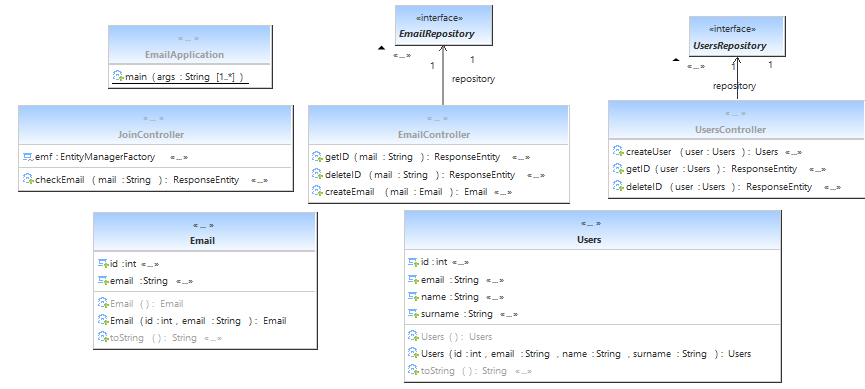
\includegraphics{img/uml}}
% 	\caption{Schema di comunicazione Utente - microservizio}
% 	\label{fig:one}
% \end{figure}

\section{Introduzione a Kong Gateway}\label{sec:kongprog}
Come accennato nel paragrafo \ref{sec:kongintro}, \emph{Kong Gateway} è un API gateway cloud-native che fornisce l’opportunità di configurare \emph{services} e \emph{routes} e, oltre a questi, anche \emph{plugin} e \emph{consumer}.
\subsection{Service}\label{sec:kongservice}
Un \emph{service} in Kong Gateway è un’astrazione di tutti i servizi upstream custom che si aggiungono alla configurazione. Con \emph{servizio upstream custom} si intende un microservizio custom che prende dati dalla richiesta inoltrata al gateway e ne restituisce altri al gateway stesso, che si occuperà di comunicarli al client.\\
Solitamente ad ogni \emph{service} è associata una o più \emph{routes}.\\

\subsection{Route}\label{sec:kongroute}
Una \emph{route} è una regola definita per indirizzare correttamente le richieste del client.\\
L’associazione di una (o più) route ad un servizio consente di realizzare un meccanismo di routing molto potente, dato che è possibile configurare nel dettaglio il percorso che si vuole realizzare (protocolli da utilizzare, livello di sicurezza ecc.).\\

\subsection{Plugin}\label{sec:kongplugin}
Un \emph{plugin} è un’entità che sarà eseguita durante tutto il ciclo di vita di una richiesta o risposta HTTP/S (HyperText Trasfer Protocol / Secure).\\
È il modo in cui Kong Gateway fornisce la possibilità di ottenere funzionalità aggiuntive per un \emph{service} o una \emph{route}.\\
I plugin possono configurabili possono essere sia proprietari (attivabili da Kong Manager) sia custom. Per la realizzazione di un plugin custom si ha la possibilità di scegliere tra vari linguaggi di programmazione per lo sviluppo quali Go, Python, JavaScript e Lua (linguaggio utilizzato per lo sviluppo del plugin custom utilizzato nel progetto).\\ 

\subsection{Consumer}\label{sec:kongconsumer}
Un \emph{consumer} in Kong Gateway può essere inteso come un utente di uno specifico servizio e può essere identificato tramite un \texttt{id} univoco.

\section{Architettura del plugin}\label{sec:architetturaplugin}
\subsection{Sviluppo}\label{sec:sviluppoplugin}

\section{Configurazione Kong Gateway}\label{sec:kongconf}